\chapter{INTRODUCTION}
\section{Background}\label{sec:background} %pelabelan ini opsional, biar bisa di klik kalo mengarahkan ke section tertentu.
\noindent Partial differential equations (PDE) are a common tool widely used in the modern scientific understanding and many engineering processes. This is because many systems can be described by the way they change and often this can be more intuitive. As an example, think of someone heating up a large frying pan on a gas stove. To describe how the pan heats up when the center is right above the burner, one can say that the center would heat up first followed by its surroundings. Eventually the pan would not heat up any further. Also notice that the edges of the pan would always be cooler than the center. However, once a more complex setup is introduced such as an uneven heat source or more complex materials with different heat rates of transferring heat it becomes much harder to describe how the pan heats up. A more useful way to describe the system is using the heat equation. For a temperature function \(u\left(\vb{x},t\right)\) of spatial coordinates vector \(\vb{x}\) and time \(t\), the generalized heat equation is defined in \cref{eq:heat_equation}.
\begin{equation} \label{eq:heat_equation}
    \pdv{u}{t}=\divergence{\left(\alpha \gradient u\right)}
\end{equation}
The divergence operator \(\divergence \) denotes sum of all first spatial derivatives. In three dimensions this is \(\divergence=\pdv{\cdot}{x_1}+\pdv{\cdot}{x_2}+\pdv{\cdot}{x_3}\). And the gradient operator \(\gradient \) is the vector of all first spatial derivatives which in three dimensions is \(\gradient{f} = {\begin{bmatrix}\pdv{f}{x_1} & \pdv{f}{x_2} & \pdv{f}{x_3}\end{bmatrix}}^{\intercal}\). This equation says that the rate at which the temperature changes in time \(\pdv{u}{t}\) is proportional to how different the differences in temperature of a spot in the pan with its surroundings \(\laplacian{u}\) multiplied with thermal diffusivity parameter \(\alpha \). One example of an insight this gives is that given a homogeneous material (\(\alpha \) is constant) and the stove outputs heat at a constant rate the temperature will no longer change for a particular point once the temperature difference is constant. In other words once the function \(u\left(\vb{x},t\right)\) at some time \(t > 0 \) approaches a linear function in space, the temperature at all spots will no longer change in time. Mathematically this is because the time derivative is zero if the second spatial derivatives are also zero. Intuitively this is because once the temperature distribution approaches linear, the current spot on the pan is outputting as much heat it is getting. This insight is an example of why PDEs are usefull.

Many other fields in physics such as waves, quantum dynamics, fluid dynamics, elastics, and many more also define systems using PDEs. PDEs are also used outside the physical sciences. In Finance, the Black-Scholes-Merton or Black-Scholes equation models the dynamics of the financial market. In ecology, PDEs are used to model population growth which is useful for modelling location dependent carrying capacity. This is used to model species distribution which can help develop better conservation policies. In the social sciences, PDEs such as the cross-diffusion model is used to explore the evolution of the urban environment \autocite{jinDetectingInteractionUrban2023}. Crowd dynamics is another field where researchers have found it useful to model using PDEs \autocite{mukherjeeLagrangianApproachModeling2015,hughesFlowLargeCrowds2000}. These are used to model dynamics such as shock-waves, pathing, and crowd flow as a whole. There are a variety of applications, ranging from bird flocks, pedestrian crowds, to robotic swarms \autocite{gongCrowdDynamicsModeling2023}.

The scenario in which PDEs are used to simulate a system typically means computing an unknown quantity like the temperature field of an object over time from a set of known parameters such as initial conditions and material parameters such as thermal diffusivity in the case of the heat equation. This scenario is termed the forward problem. The inverse problem on the other hand solves for an unknown parameter using other known parameters and observations of the partial solution such as temperature field at the object's surface. Traditional methods used to solve these problems utilized knowledge of the exact equations to numerically solve PDEs. As an example, the Finite Difference Method (FDM) approximates the solution by substituting the partial derivatives with finite differences such as the first derivative approximation in \cref{eq:forward_finite_difference_1}.
\begin{equation} \label{eq:forward_finite_difference_1}
    \pdv{f\left(x\right)}{x} \approx \frac{f\left(x+h\right)-f\left(x\right)}{h}
\end{equation}

Traditional numerical solvers have enjoyed many decades of development due to their long history. There are many general approaches to solve PDEs and many more very specific approaches. Other than FDM, some widely used approaches include Finite Element Methods (FEM), Finite Volume Methods (FVM), Collocation Methods, and Spectral Methods. FEM and FDM are both mesh based approaches, meaning they rely on discretization of the computational domain <ADD DIAGRAM FOR THIS>. There are several challenges associated with this. First, irregular domains such as bone, spider silk, gravel, or other bio-inspired or aggregate materials pose a challenge due to the complexity of the domain geometry \autocite{gaulSimulationWavePropagation1991,buoniEfficientScalableNumerical2007,jiaModulateStressDistribution2024}. Also, irregular domains which create large deformations or mesh entanglement cause these methods to become ineffective \autocite{chenMeshfreeMethodsProgress2017}. While there are strategies to mitigate this, by definition they are an additional layer of difficulty to the process. Second, multiscale applications where the micro and macro scales are both important require fine meshes such that the small scale structures are adequately simulated. This creates meshes with very large number of points that are very resource intensive \autocite{buoniEfficientScalableNumerical2007}. Therefore, in problems where these issues important or resources are limited, mesh-free methods are preferred. Third, traditional methods require prior knowledge of analytic forms of PDEs. This is because the solvers use the equations to formulate the solution. A dealbreaker like this makes traditional numerical approaches unsuited to data dominant problems. Fourth, a single evaluation of traditional solvers may not be very costly, however multiple evaluations can add up. This is very apparent in inverse problems where the solver is evaluated multiple times to compute gradients in order to obtain parameter functions. These challenges altogether have motivated research into alternative methods that do not completely rely on prior knowledge, mesh free, and fast enough when computing solutions from parameters.

With the increasing prevalence of machine learning methods and their use in more and more fields, research into their use for scientific computing has taken off in recent years. While statistical modeling has already been widely used in areas such as physical constants, stellar population studies, risk assessments of events such as earthquakes and coronal mass ejections \autocite{berlinerPhysicalStatisticalModeling2003,anselmoComputationalMethodsReentry2005,reinhardtAsteroidRiskAssessment2016,uzanFundamentalConstantsTheir2003,spanosWhereStatisticalModels2006,bernardiStellarPopulationAnalysis2022}, the dominant approach for forward modeling or inverse modeling has remained physics based numerical models. Machine learning has provided an alternative approach to model the solutions of PDEs. In their work, \textcite{aartsNeuralNetworkMethod2001} utilized neural networks to approximate each term of PDEs describing damped and undamped free vibrations and substituting them into the PDEs and associated initial conditions. The network parameters were then optimized to reduce the PDE residual and boundary condition loss using evolutionary algorithms. This approach was taken in order to make machine learning models more transparent which at the time was being pursued because of the high cost of optimizing uncertainties in water management numerical simulators. However, since this method approximates the mapping between coordinates and the values of a function and their derivatives, retraining would be necessary for changes to the function itself. This could become very costly as retraining costs accumulate. A more recent approach that also utilizes soft constrains from PDE residuals is termed physics informed neural network (PINN) \autocite{raissiPhysicsinformedNeuralNetworks2019}. The authors propose a framework that leverages advancements in computing, namely automatic differentiation (AD) techniques made readily available by modern machine learning libraries. In general, PINNs use AD to compute each term of the PDE from the output of the model and this is then substituted into the PDE to in order to compute the residuals and loss from boundary conditions. The network residual and boundary loss are then weighted and summed with the data loss. For a neural network \(\hat{u}\left(\vb{x},t\right)\) approximating the real solution \(u\left(\vb{x},t\right)\), the residual loss for the heat equation in \cref{eq:heat_equation} is \cref{eq:heat_pinn_loss}. One issue with using AD to compute the residual is that the network input needs to be the independent variable (i.e.\ coordinates, time, etc.). This once again means that if one wants to compute a different solution, the network needs to be retrained.
\begin{equation}\label{eq:heat_pinn_loss}
    \mathcal{L}_{PDE}={\left(\pdv{\hat{u}\left(\vb{x},t\right)}{t}-\divergence{\left(\alpha \gradient \hat{u}\left(\vb{x},t\right)\right)}\right)}^2
\end{equation}
Other works utilize convolutional neural networks (CNN) to compute the solution from input functions such as forcing terms or initial conditions. This approach generally means discretizing the functions on a grid and using these as training data. One study by \textcite{wangPhysicsinformedDeepLearning2020} predicts turbulent flow using spatial and temporal decomposition and a specialized U-Net, an architecture based on CNNs, to predict the velocity field from the decomposition of the previous velocity field. Part of the loss function is a regularization term for zero divergence in the velocity field to enforce incompressible fluid flow. This term was calculated using finite differences since auto differentiation is not applicable in this situation. Finite differences was also utilized in another CNN based fluid flow upscaling model by \textcite{gaoSuperresolutionDenoisingFluid2021} to compute the residual terms of the steady incompressible Navier-Stokes equation. This model also inferred unknown physical parameters such as boundary conditions. However, this approach would mean the model would need to scale as a quadratic in 2D, cubic in 3D, and much steeper in higher dimensions. Outside fluid dynamics, the combination of specialized CNNs and finite differences or another numerical differentiation method have been used for many other PDEs including Poisson's equation for temperature fields \autocite{zhaoPhysicsinformedConvolutionalNeural2023, gaoPhyGeoNetPhysicsinformedGeometryadaptive2021}, velocity models from seismic data \autocite{mullerDeepPretrainedFWI2023}, and seismic response of structures \autocite{zhangPhysicsguidedConvolutionalNeural2020,niMultiEndPhysicsInformedDeep2022}. While the use of CNNs mean that discretization is implied, solutions of different initial conditions or parameter functions can be computed by inference and no retraining is required.

The mapping between discretized functions done by CNNs are related to an alternative approach that starts by viewing PDEs as operators, which are generalized mappings between spaces. One group of familiar operators are functions which maps between spaces of scalar values or vector values. PDEs on the other hand are operators that map between function spaces. A simple example is the derivative. The derivative takes in a function and returns the derivative of said function. In other words it is an operator that maps between the space of all functions to the space of derivatives of those functions. Another way to view operators starts by viewing functions as infinite dimensional vectors. Where elements in the vector are the function's value evaluated at every point in space. The operator can be seen as a vector function mapping between these infinite dimensional vector spaces. Operators are important because a field of research has sprung up around this mathematical concept. Operator learning is the use of machine learning to learn operators using data driven approaches. As an analogy, function regression traditionally has been used to approximate the mapping between input values such as coordinates and output values of functions evaluated at said coordinates. In the case of operator learning, the mapping between function spaces are approximated. The aforementioned approaches using CNNs does this directly using the values of functions at discrete points. There are other approaches like DeepONet that does not require the uniform grid like CNNs \autocite{luLearningNonlinearOperators2021}. This architecture instead uses both input functions and coordinates as inputs. The output is the output function evaluated at the coordinates provided. This architecture is based on an extension for deep learning of the universal operator approximation theory for neural networks first proposed almost three decades ago at the time of writing by \textcite{chenUniversalApproximationNonlinear1995}. The proposed architecture is composed of two sub-networks, where one termed the trunk \(\hat{\vb{T}}\left(\vb{x},t\right)\)learns the latent mapping for coordinates and the other network termed the branch \(\hat{\vb{B}}\left(\vb{f}\right)\) learns the latent mapping for the input function \(f \). The two latent mappings are combined through a dot product to obtain the approximated output function value \(u \left( \vb{x}, t \right)\). This is formulated in \cref{eq:universal_op_approx_nn}.
\begin{equation}\label{eq:universal_op_approx_nn}
    u\left( \vb{x}, t \right) \approx \hat{G}\left( \vb{f} \right)\left( \vb{x}, t \right) = \hat{\vb{B}}\left( \vb{f} \right) \cdot \hat{\vb{T}}\left( \vb{x}, t \right)
\end{equation}
Fourier Neural Operators is an alternative avenue for learning operators by utilizing the fact that functions can be decomposed into linear combinations of basis functions, namely trigonometric basis in this particular case \autocite{li2021fourier}. With this method the input function value is mapped to its corresponding output function value. This is done by first lifting the input function value to a higher dimension using a neural network and this is then passed through blocks composed of a Fourier transform, then a linear transform and filtering of higher modes, and finally the inverse Fourier transform. These blocks are stacked to a desired depth and finally another network projects the outputs to the target dimension. The reason a linear can be used is that differentiation is multiplication in the Fourier domain. One drawback with FNO is the requirement that output functions are not parameterized by coordinates and therefore is implicitly relative to the input function coordinates. To avoid this issue, \textcite{fanaskovSpectralNeuralOperators2023} reframes the problem by directly utilizing the coefficients of the input function computed using Fourier transform to predict the coefficients of the output function in terms of coefficients a Fourier series.

\noindent Non-destructive testing (NDT) is critical process in the field of engineering and quality assurance that allows the evaluation of a subject without causing damage \autocite{howell2020nondestructive, maioUltrasoundPropagationComposite2022, bochudSparseDigitalSignal2015}. This makes NDT crucial in many cases like construction and manufacturing where testing needs to be done on products without damaging it. The use of NDT allows for early detection of flaws and anomalies ensuring the reliability, longevity, and safety of structures and machinery. A widely used form of NDT, ultrasonic testing, propagates mechanical waves into the material. The ultrasonic waves, typically in the kHz to MHz range, travel through the material and interact with inhomogeneities in the material i.e. waves reflected by a cavity. This makes it possible to determine the location, size, and nature of deformities by analyzing the waves measured at predetermined locations. The measurements themselves result in a time series of wave amplitudes represented as displacement. The data can be presented as shown in \Cref{fig:us_presentation}. The amplitude time series by itself is referred as an A-Scan. B-Scans take measurements at multiple locations to show a cross-section of the subject. C-Scans adds another dimension of measurements and presents a view of things that reflect the waves such as defects. Analysis of the ultrasonic data can then be carried out. When the material can be assumed homogeneous, ray based or time of flight based methods can be used. In pulse echo, the wave travels through the material and gets reflected by interfaces, whether the other side of the material, fractures within, or generally modulus/density discontinuities present in the material. This means the measurements would record a large amplitude initially from the impulse sent into the material. And then the reflected waves from the closest interface would arrive. This way, just by knowing the exact wave speed of the material, one could easily translate reflected wave arrival time into the positions of interfaces.

\begin{figure}[ht]
    \centering
    \includesvg[inkscapelatex=false, width=1.0\linewidth]{gambar/us scan presentations}
    %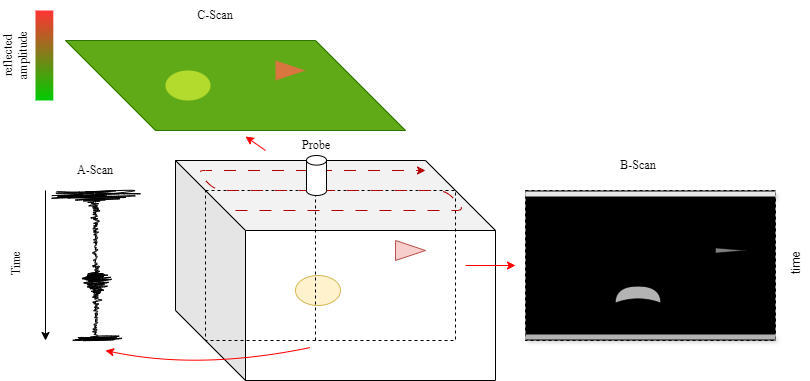
\includegraphics[width=1.0\linewidth]{gambar/us scan presentations.png}
    \caption{Different presentations of ultrasonic scan data. The subject is a box containing several anomalies indicated by the yellow oval and red triangle. The fist presentation is the A-Scan where the amplitude measured over time in one location. The second is B-Scan where the amplitudes over time is measured along a line. The results are then stacked with the vertical axis acting as time and the horizontal axis as position. The higher amplitudes correspond to lighter pixels. The third presentation is C-Scan which is a view of the amplitudes of reflected waves except the initial impulse and back wall reflection.}
    \label{fig:us_presentation}
\end{figure}

Ultrasonic NDT has advantages that make it one of the more widely used NDT methods \autocite{howell2020nondestructive, nivenFullWaveformInversion2020, feliceSizingFlawsUsing2018}. One advantage is that ultrasonic testing equipment is often portable making it suitable for cases where it is difficult or not possible to test in a controlled environment such as a laboratory. Inspections for infrastructure such as pipes or rail tracks are examples where it is costly and very disruptive to move the test subject to a testing location \autocite{}. Another advantage of ultrasonic testing is the low risk it poses in terms of safety. Unlike the ionizing radiation used in radiography, ultrasonic waves used in testing are harmless to humans. This means testing can be done with relatively less stringent safety precautions \autocite{}. Additionally, the technology is relatively mature with a variety of equipment and supplier options. Furthermore, affordable options for inexpensive ultrasonic equipment is also available \autocite{}. These advantages and the popularity of ultrasonic testing stemming from the aforementioned advantages highlights the important role ultrasonic testing plays in enabling affordable and reliable engineering.

%Talk about the process of A-scans, B-scans, C-scans. Talk about why its hard to analyze for more complex situations which are gaining popularity ie. composites.

The emergence of composites, sought after for their multi-functional properties, introduces challenges for inspection and analysis \autocites{inceOverviewEmergingHybrid2023, yangUltrasonicDetectionMethods2023, dwivediAdvancesResearchesNon2018, nivenFullWaveformInversion2020}. Different composites provide a range of benefits, from the strength to weight ratio of carbon fiber reinforced polymer composites to electromagnetic shielding materials. However, the anisotropic and complex characteristic of composites that give rise to the beneficial properties complicates wave propagation because of the location and directional dependence of material properties. For example wave speed can be faster in certain directions and locations. Reflections will happen not just because of anomalies, but also expected features in the material itself. Extraneous signals from inhomogeneities anticipated in the material makes it harder to extract useful information on unknown defects. In order to enable reliable use of ultrasonic NDT on composite materials and other complex situations, a method to quantify and characterize the complicated behavior is required \autocite{maioUltrasoundPropagationComposite2022}.

This is where model based methods come into play. Advances in computation over recent decades has enabled the use of computational tools to revolutionize many fields. Numerical modeling, in particular, has an almost symbiotic relationship with the rise of computing; with the likes of ENIAC, MANIAC, and a plethora of other early electronic digital computers \autocite{andersonScientificUsesMANIAC1986}. The ENIAC for example, promised to compute ballistic trajectories 10 times faster than the methods that were in used at the time. This progress allows the simulation and analysis of systems previously beyond reach. The effects range from prediction of weather systems and physics constrained problems like bleeding edge aerospace design to uncovering physical laws of nature.

Despite advances in computing power, numerical modeling of physical systems still remains an open problem with many challenges. Traditional methods such as Finite Element Method (FEM), Finite Difference Method (FDM), and Spectral Methods are limited to known operators and equations \autocite{karniadakisPhysicsinformedMachineLearning2021, du2024neural,fanaskovSpectralNeuralOperators2023,luLearningNonlinearOperators2021}. The modern data landscape further complicates traditional numerical modeling with its characteristic abundance of low quality, high quantity data, as some methods such as FDM are inherently sensitive to noise \autocite{dearagaoExplicitControlNumerical2021, huntulInverseProblemReconstructing2021}. Noisy data also presents a formidable challenge in general because gleaning any meaningful information from noisy and incomplete data requires further filtering and interpretation. This issue is particularly troubling for inverse problems. This is because some inverse problems are unstable in addition to their ill-posedness which necessitates advanced techniques \autocite{caubetInstabilityInverseProblem2013, mandacheExponentialInstabilityInverse2001}. The next layer of complexity is posed by the challenge of irregular domains. An example of this is fluid flow through materials such as gravel, sponges, even changing with time \autocite{liImmersedInterfaceMethod2006}. Due to the nature of irregular domains, mesh based methods struggle to adapt. Addressing these challenges is crucial for understanding a variety of problems in both scientific research and engineering.

%talk more about each challenge and the proposed solutions to it and how they do not fully cover the needs this work is trying to cover
The problem posed by model-based ultrasonic testing combines several of these challenges. First, visualizing properties of materials such as density from measurements of ultrasonic waves that interacted with the material is an inverse problem. This is because the effect is used to infer the cause. The challenge with inverse problems is that in many cases, the result is very sensitive to differences in the parameters \autocite{tarantolaInverseProblemTheory2005}; small variation in density distribution can result in very different measurements. As such, additional noise or inaccuracies in measurement can massively impact the predicted parameter. This very issue has been a long standing challenge in the geophysics community. The full waveform inversion (FWI) procedure used to determine properties of the earth, requires certain techniques such as a minimization criteria that mitigates this sensitivity \autocite{virieuxOverviewFullwaveformInversion2009}. Second, complex or irregular domains are a challenge for traditional mesh based methods as the domain may vary in time \autocite{liImmersedInterfaceMethod2006, burchnerImmersedBoundaryParametrizations2023}. Costly mesh generation hampers the performance of mesh based methods. In addition, some approaches like total focusing method (TFM), traveltime tomography (TT) and reverse time migration (RTM) are not able to provide more than a rough estimate of defects. Third, for some materials, there are little to no knowledge present in literature on how waves propagate through the material. Continued research has alleviated this issue by advanced our understanding of wave propagation and materials. \textcite{gordoaUltrasonicWavesBubbly2021} presented an analytic solution to ultrasonic wave propagation in bubbly liquids. \textcite{} . However, these solutions are not available for all situations and materials, as such is the case when a novel material is created. In some of these cases data collection may be easier to do compared to deriving from first principles.

%Talk about how composites, ndt, rapid prototyping, bigalow inflatable space habitat, etc is important to aerospace
Advances in computing technology and the integration of non-destructive testing have revolutionized the aerospace industry \autocite{guptaAdvancesApplicationsNonDestructive2022, jacobDataFusionEfficient2022}. This has had the effect of enabling rapid advancements in cutting-edge technologies such as vertical rocket landings, 3-D printed spacecraft, and in-space manufacturing to name a few \autocite{corradoSpaceExplorationEconomic2023}. These technologies addressed several key challenges with space exploration, namely cost, mission flexibility \& resilience, and environmental considerations. NDT plays a crucial role in ensuring the safety and quality of the innovations. The novelty of innovations means they do not have the luxury of being a proven solution.

%Talk about related works, using conventional methods, using nn, using other machine learning methods, using spectral methods.

Bagian ini mendeskripsikan gambaran umum, konteks, dan posisi penelitian TA dalam konstelasi perkembangan pengetahuan yang telah dicapai. Penjelasan yang dituliskan menjadi penting karena dengan landasan yang kuat, maka pekerjaan penelitian dapat terarah dilakukan. Hal ini lebih spesifik dan tegas disampaikan pada sub-sub bab berikutnya.

Beberapa pustaka utama yang berperan dominan dapat disampaikan di sini untuk memberi gambaran tentang letak penelitian TA dalam konstelasi keilmuan yang dicapai. Hasil-hasil dari pustaka terbaru dapat menopang Latar Belakang ini menjadi lebih kuat.

Sangat wajar apabila isi sub bab setelah Latar Belakang ini mengalami penyesuaian saat sejumlah hasil penelitian sudah diperoleh dan dianalisis. Pada dasarnya, hal ini dimungkinkan apabila ada penyesuaian kecil, karena fokus penelitian sejatinya sudah jelas sedari awal, namun hasil-hasil yang diperoleh dapat memperbaharui beberapa butir isi sub bab. Oleh karena itu, finalisasi isi Pendahuluan ini biasanya dilakukan menjelang akhir pembuatan laporan penelitian yang dituangkan dalam buku TA.


\section{Rumusan dan Batasan Masalah}
\noindent Bagian ini menjadi salah satu bagian penting dalam Pendahuluan. Setelah paparan Latar Belakang, maka masalah yang diangkat pada pekerjaan penelitian perlu dirumuskan dengan baik. Perumusan ini sebaiknya dibahasakan tidak dalam bentuk kalimat pertanyaan, melainkan kalimat aktif, dan dapat memuat lebih dari satu rumusan.

Sejalan dengan ini, setiap masalah yang diangkat selalu memiliki batas. Ada batasan, asumsi, atau kriteria yang menjadi pembatas atas masalah yang diangkat dalam penelitian TA, sehingga arah penelitian dapat fokus. Batasan ini perlu dituliskan secara tegas, dan dapat saja memuat lebih dari satu.


\section{Tujuan}
\label{sec:tujuan}
Bagian ini secara tegas menuliskan tujuan pekerjaan penelitian TA, yang dapat memuat lebih dari satu. Pemilihan kata kerja pada Tujuan ini sangat penting karena menggambarkan arah fokus dari jalinan upaya yang dilakukan.


\section{Metodologi}
Di sini disampaikan metodologi yang diterapkan pada pekerjaan penelitian TA. Beberpa di antaranya adalah pengamatan dan akuisisi data, eksperimen numerik, studi pustaka, teoretik atau analitik, dan semi analitik dengan komplemen numerik.



\section{Sistematika Penulisan}
\noindent Bagian ini adalah penutup Bab I yang menyampaikan  secara ringkas isi setiap  bab. Karena pembaca sudah sampai akhir Bab I, yang  berarti  sudah  mengetahui isinya, maka tidak perlu ditulis lagi rincian Bab I. Sebaiknya langsung dituliskan secara ringkas isi rincian bab-bab selanjutnya, misalnya, \textit{Setelah Pendahuluan pada Bab I ini, Bab II akan mengulas tentang ...}

Apabila diperlukan, dapat dituliskan konvensi khusus yang digunakan pada penulisan naskah buku TA ini, misalnya tanda titik menggantikan tanda desimal karena alasan kemudahan dan kejelasan dalam formulasi matematika.